\section{Introduction}
\begin{figure}
	\centering
	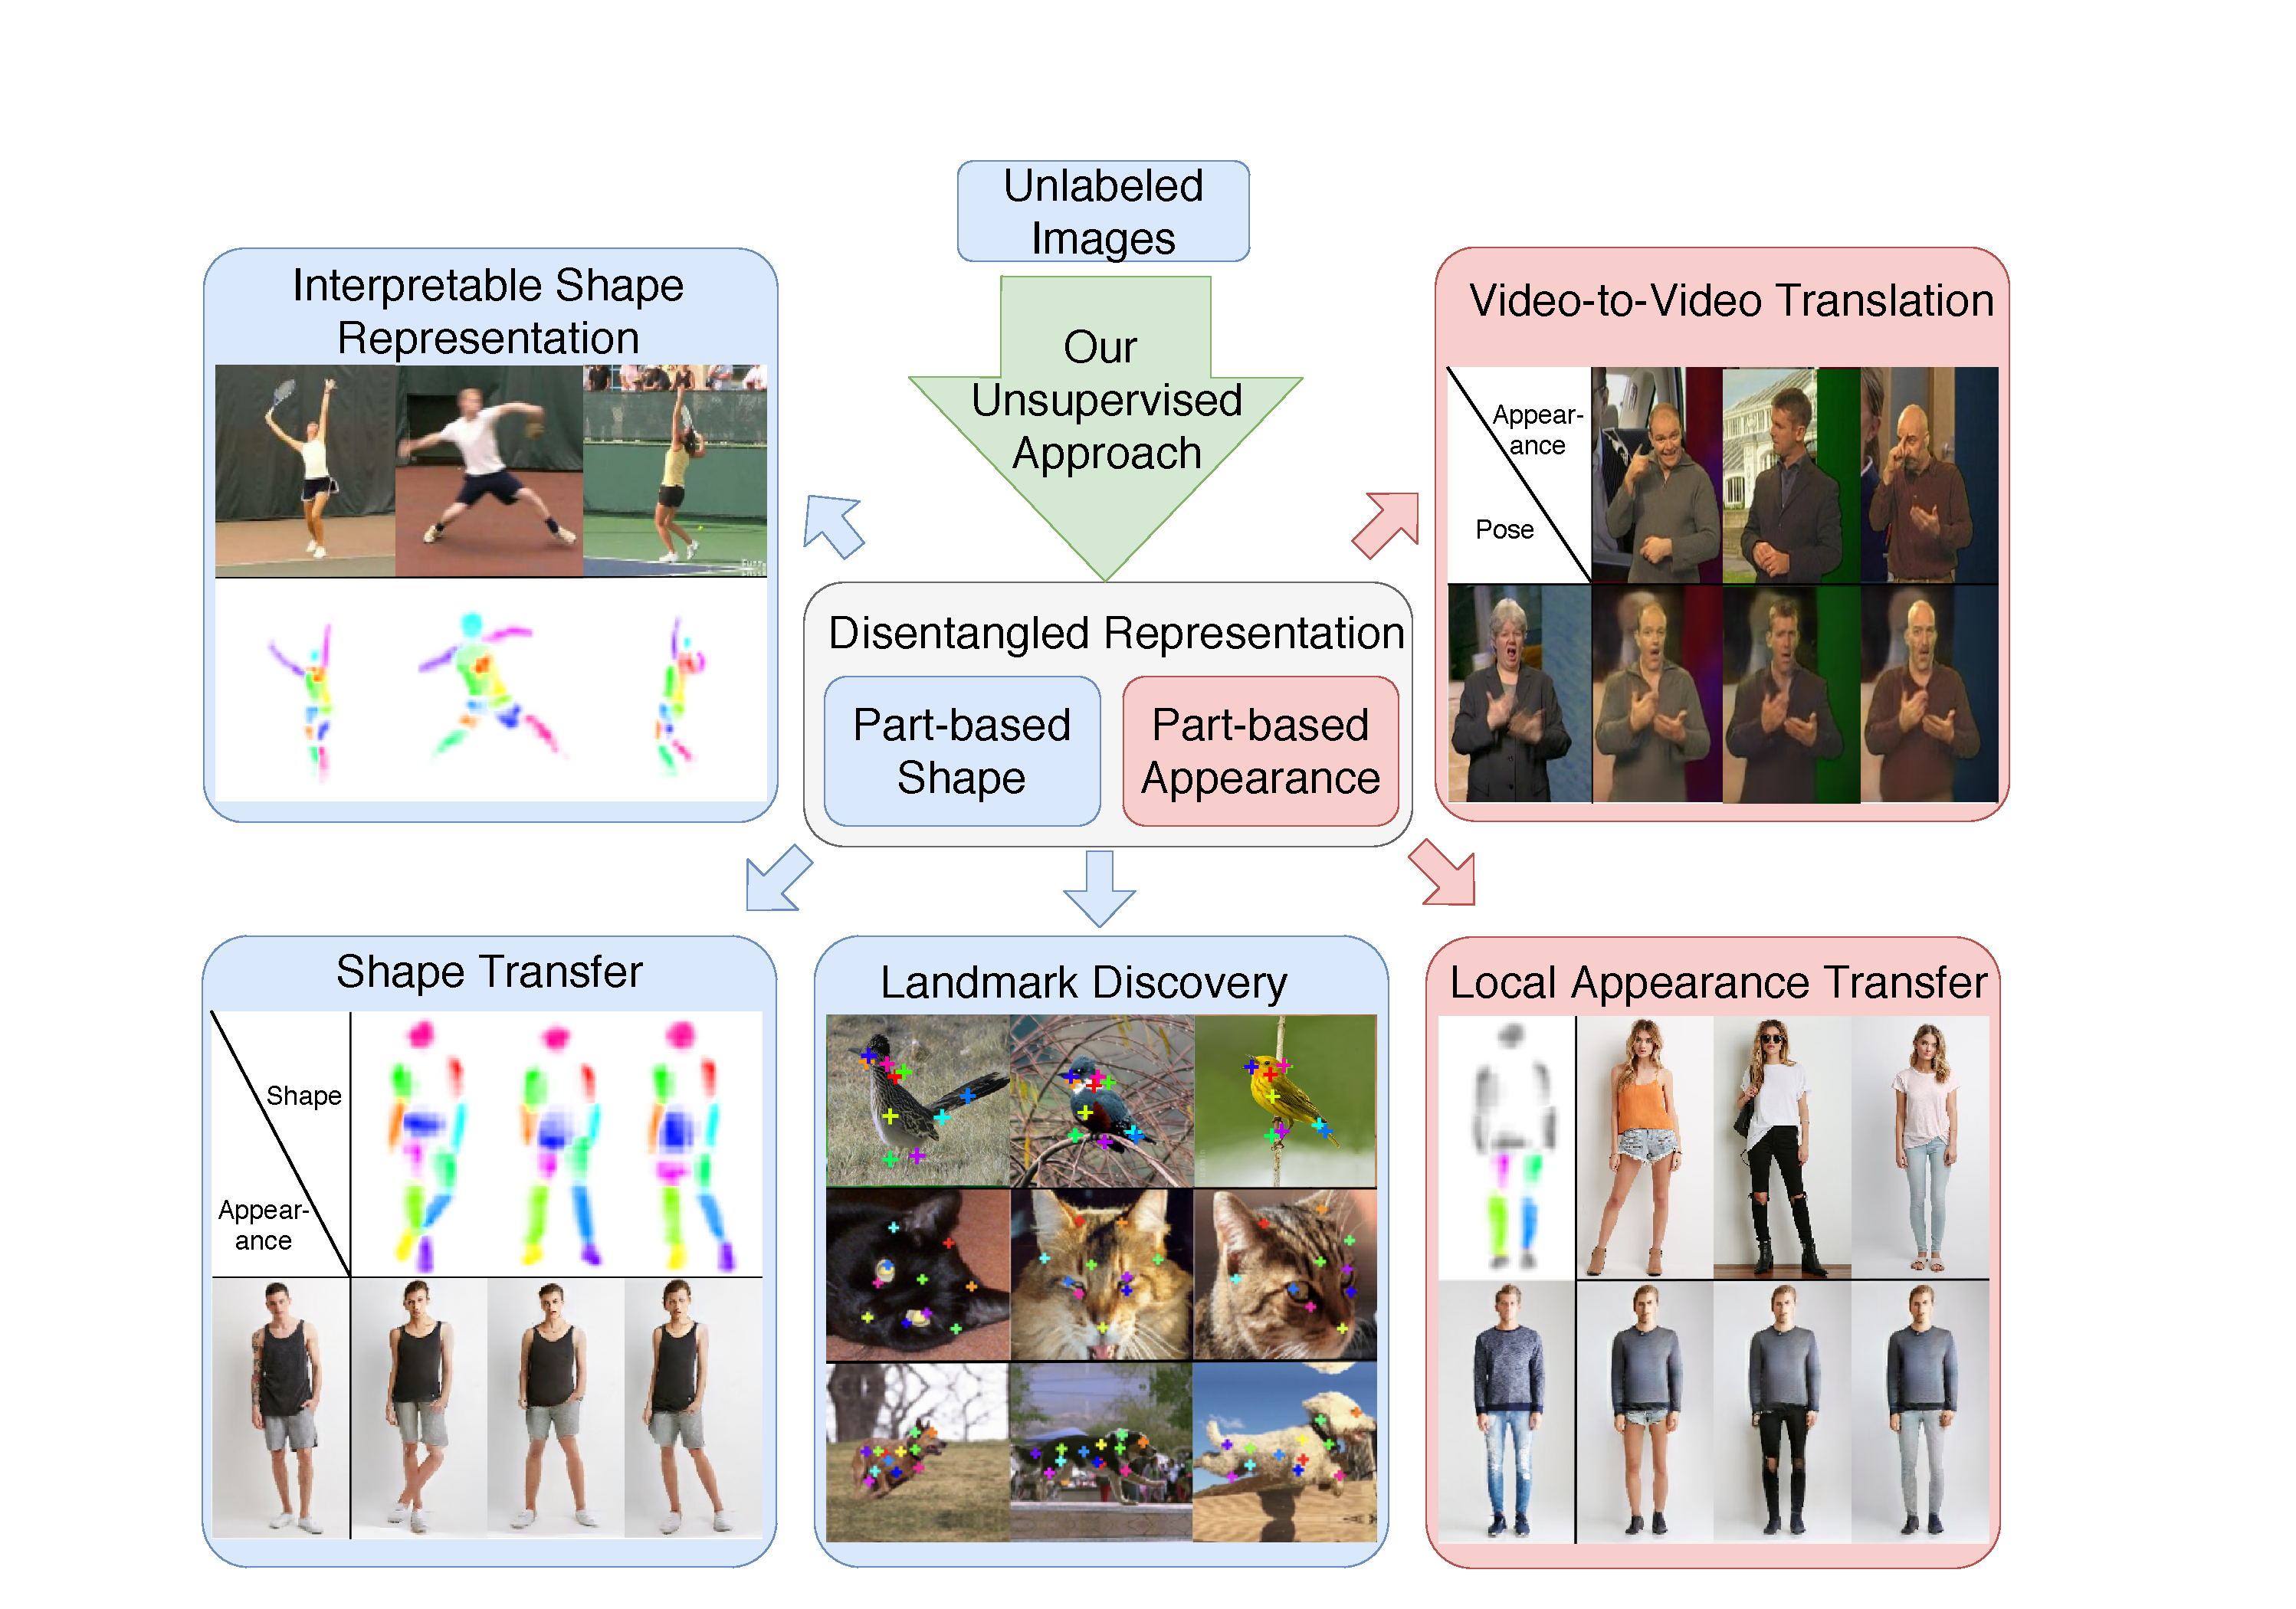
\includegraphics[trim={4.5cm 0.5cm 6.3cm 0cm},clip, width=1.\linewidth]{fig/front_final.pdf}
	\caption{Our unsupervised learning of a disentangled part-based shape and appearance enables numerous tasks ranging from unsupervised pose estimation to image synthesis and retargeting.} % for an object class}
	\label{fig:firstpage}
\end{figure}

A grand goal of computer vision is to automatically, without supervision information, learn about the characteristics of an object in the world.  Typically, images show the interplay of multiple such factors of variation. We
%then
want to disentangle \cite{Desjardins2012dr, Bengio2013rep, Chen2016infogan, Higgins2016betavae, Eastwood2018dr} the effects of these different characteristics and imagine, i.e., synthesize, new images where they are altered individually. For instance, after observing a number of different unlabeled instances of an object category, we want to learn their variations in shape (such as pose relative to the viewer and body articulation) and appearance, \eg, texture and color differences in fur/clothing or skin color. Disentangling shape and appearance is particularly challenging because object deformation typically leads to complicated
\enquote{recoloring} of image pixels \cite{Shu:2018ua,Esser:2018ue}: moving a limb may change the color of former background pixels into foreground and vice versa.

To address the disentangling problem for shape and appearance, several supervised methods have been proposed lately~\cite{Ma:2017wq, Ma:2017uu, deBem:2018wp, Esser:2018ue, Siarohin:2018wk, Balakrishnan:2018wo}. By conditioning generative models on a pre-specified shape representation, they are able to successfully explain away appearance. However, they are limited to object categories, for which pose labels are readily available such as human bodies and faces, but they cannot be applied to the vast amounts of unlabelled data of arbitrary object classes.

For unsupervised learning, instead of taking a known shape to capture all non-shape factors, both shape and appearance need to be learned  simultaneously.
Recently some unsupervised approaches have been proposed to disentangle these factors~\cite{Shu:2018ua, Xing:2018un}. However, these works have only shown results for rather rigid objects, like human faces or require several instances of the same person \cite{Denton:2017uf}.

Object variation can be global, such as difference in viewpoint, but it is oftentimes local (animal tilting its head, person with/without jacket), thus calling for a local, disentangled object representation. %instead of recent holistic disentangling models~\cite{Esser:2018ue, Ma:2017wq, deBem:2018wp, Ma:2017uu}.
The traditional answer are compositions of rigid parts~\cite{Fischler1973rep, Fergus2003object, Felzenszwalb:2010ve}.
In the context of recent unsupervised shape learning an instantiation
of this are landmarks~\cite{Thewlis:2017wi, Zhang:2018vz, Jakab:2018wc}. % which have shown promising results for representing shape. % Thus, we disentangle on the level of parts.
% In addition, to disentangle, we also model the extend of a part and add a local part appearance representation. % In order to reach a disentanglement, we also model the extend of a part and add a local part appearance representation.

In this paper, we propose the first approach to learn a part-based disentangled representation of shape \textit{and} appearance for articulated object classes %based only on single images
without supervision and from scratch.
In the spirit of analysis-by-synthesis~\cite{Yildirim:2015ur}, we learn the factors by a generative process.
We formulate %derive
explicit equivariance and invariance constraints an object representation should fulfill
and incorporate them in a fully differentiable autoencoding framework.

Our approach yields significant improvements upon the state-of-the-art in unsupervised object shape learning, evaluated on the task of landmark regression.
We compare to competitors on a wide range of diverse datasets both for rigid and articulated objects, with particularly large gains for strong articulations.
Furthermore, our disentangled representation of shape and appearance competes favorably even against state-of-the-art supervised results.
We also show disentangling results on the task of video-to-video translation, where fine-grained articulation is smoothly and consistently translated on a frame-to-frame level.
Lastly, since our representation captures appearance locally, it is also possible to transfer
%and manipulate
appearance on the level of individual object parts. An overview of the scope of possible applications is given in Fig.~\ref{fig:firstpage}.
